\begin{savequote}[75mm] 
The journey of a thousand miles begins with one step.
\qauthor{Lao Tzu} 
\end{savequote}

\chapter{Topic clustering and classification (TCC) for multilingual ATS}
\label{chap:tcc}


Clustering has been used for summarization in many systems, either using documents as units, sentences or words. 
The resulted clusters are used to extract the summary.
Some systems use just the biggest cluster to score sentences and get the top ones such as `UoEssex" system \citep{11-elhaj-al} which is justified by the assumption that a single cluster will give a coherent summary. 
Others take a representative sentence from each cluster, in order to cover all topics. 
While there are systems which score sentences according to all clusters.
%scoring
These three methods represent how each sentence is selected to be in the summary based on its cluster(s). 
But to score these sentences, we can divide the scoring methods into two groups: rule based and data driven. 
The former one rely on hand written rules to score sentences. % such as in ``CIST" and ``UoEssex" systems.
%``CIST" \citep{11-liu-al,13-li-al} uses \ac{hlda} model to cluster sentences into sub-topics.
%Then, the sentences of the largest sub-topic are scored using \ac{hlda} model combined with some traditional features. 
%Likewise, ``UoEssex" \citep{11-elhaj-al} uses K-Means to cluster similar sentences.
%Sentences of biggest cluster are scored using their cosine similarities to the cluster's centroid. 
On the other hand, data driven methods use machine learning to infer scoring or decision models. 
%For instance, ``CLASSY" system \citep{11-conroy-al} uses na\"ive Bayes to estimate the log-likelihood that a term may be included in the summary.

%Problems facing multilingual summarization
One of multilingual summarization's problem is the lack of resources such as labeled corpus used for training.
Machine learning algorithms were used either to select the sentences that should be in the summary, or to estimate the features' weights. 
Both cases need a training corpus given the language and the domain we want to adapt our summarizer to. 
To design a language-neutral summarization system, either we adapt our system to input languages (Partly language-neutral), or we design a system that can process any language (Fully language-neutral). 

In this chapter, we will present our method based on clustering and machine learning to score sentences in a multilingual fashion which is called \acf{tcc} \citep{13-aries-al,15-aries-al}. 
It will be used as a baseline in our other methods. 
%
In this method, we use a simple fuzzy clustering algorithm.
We assume that a sentence can express many topics, and therefore it can belong to many clusters.
Also, we believe that a summary must take in consideration other topics than the main one (the biggest cluster).
To score sentences, we use a scoring function based on Na\"ive Bayes classification. 
It uses the clusters for training rather than a corpus, in order to avoid the problem of language dependency.
Figure \ref{fig:gnrl-arch} represents the general architecture of AllSummarize\ac{tcc} method.

\begin{figure*}
	\begin{center}
		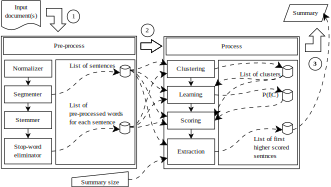
\includegraphics[width=\textwidth]{figures/tcc/gnrl-arch.pdf}
	\end{center}
	\caption{\label{fig:gnrl-arch} General architecture of AllSummarizer (TCC method).}
\end{figure*}


\section{Preprocessing}

This is the language-dependent part, which can be found in many information retrieval (IR) works. 
It is needed by the method but does not affect the fact that the method is language independent. 
Also, these tools are not difficult to be found for most languages since they are simple compared to other natural language processing tasks.
In our system, we are interested in these preprocessing tasks: Normalization, Segmentation, Stemming and Stop words removal.
%\begin{itemize}
%	\item Normalization	
%	\item Segmentation
%	\item Stemming
%	\item Stop words removal
%\end{itemize}


% Normalization
Normalization is the process of transforming a text into a canonical form. 
It is used to get one form especially for as acronyms, Abbreviations, dates and numbers. 
For instance, in a text, the author can write the number 4 as ``four" in some parts and as ``4" in others. 
In case of HTML text, tags has to be deleted before processing the text; otherwise, they will affect the task in question. 
Also, it can be used to delete special characters such  are diacritics (Tashkiil) in case of Arabic and  Persian. 
In our case, we use this task just for Arabic and Persian, since the diacritics create many variations of the same word. 
For instance, the word ``\textarab[voc]{عَمِلَ} \textit{/‘amila/ ([He] worked)}" and ``\textarab[voc]{عَمَلٌ} \textit{/‘amalun/ (work)}" can be treated as the same while processing.

% sentence segmentation
Text segmentation task is composed of two sub-tasks: sentence segmentation and words tokenization.
First of all, we must split the input text into several sentences mostly using punctuation. 
Detecting sentence boundaries using the period mark can fail when it meets some abbreviations such as: ``Dr.", ``Mr.", ``Ms.", ``PhD.", etc. 
Also, there exists some languages such as Thai which does not have a delimiter for sentences.
% words tokenization 
After segmenting each sentence apart, we must recover the list of words using a task called ``words tokenization".
Splitting a text into words is not as simple as using the blank (white space) as a separator. 
Languages such as Japanese and Chinese does not use blank character to separate the different words of a sentence. 
For instance, the Japanese sentence ``私の名前はカリムです。 \textit{/watashi no namae wa karimu desu./ (My name is Karim.)}" does not have any marks to distinguishing different words.

% stemming
Due to variations resulted from inflection or derivation of words, we end up with many variations of the same word. 
For instance, the word ``inspire" can have many derivations: ``inspirer", ``inspiration", etc. and conjugation forms: ``inspired", ``inspires".
The solution is to use stemming which aims to remove prefixes, suffixes and infixes in order to help associating variants of the same term with a common root form.

% stop words removal
Some words are better not to be included into the scoring process.
Among these words, we can mention: pronouns, prepositions, etc. which are independent from the subject of the text.
It is too easy to find a list of these words on the web for a given language.


% used tool
In our work, we use an open source tool (LangPi\footnote{LangPi: \url{https://github.com/kariminf/langpi}}) which we designed to afford these tasks for 40 languages.
Table \ref{tab:preprocess} shows each language and the tools used for each preprocessing task.
For more information about LangPi, check Appendix A.
%
\begin{table}[!ht]
	\centering
	\caption{Tools used to preprocess each language in LangPi}
	\readtable{tcc/preprocess.tex}
	\label{tab:preprocess}
\end{table}


\section{Topics clustering}

Each text contains many topics, where a topic is a set of sentences having some sort of relationship between each other.
In our case, this relationship is the cosine similarity between each two sentences. 
Which means, the sentences that have many common terms are considered as having the same topic. 
Given two sentences $ X $ and $ Y $, the cosine similarity between them is expressed by Equation \ref{eq:cosine}.

\begin{equation}
\label{eq:cosine}
cos(X,Y) = \frac {\sum_i {x_i.y_i} }
{\sqrt{\sum_i(x_i)^2} . \sqrt{\sum_i(y_i)^2}}
\end{equation}
Where $ x_i $ ($ y_i $) denotes frequencies of each term in the sentence $ X $ ($ Y $).
$x_i.y_i$ represents the multiplication of shared terms frequencies between X and Y.


To generate topics, we use a simple algorithm (see Algorithm  \ref{algo:cluster}) which is based on cosine similarity and a clustering threshold $ th $ to clustering $ n $ sentences.
The sentences having a similarity greater than $ th $ are regrouped into the same cluster. 
A sentence can belong to many clusters at once, this is motivated by the fact that a sentence can discuss many topics.

\begin{algorithm}[!ht]
	\readalgo{tcc/cluster.tex} 
	\caption{Clustering method used in AllSumarizer TCC}
	\label{algo:cluster}
\end{algorithm}



\section{TCC scoring function}

A summary is a short text that is supposed to represent most information in the source text, and cover most of its topics.
Therefore, we assume that a sentence can be in the summary when it is most probable to represent all topics (clusters)  using a set of features.
Assuming clusters independence, the probability of a sentence $ s_i $ representing all topics $ c_j \in C $ based on some features $ f_k \in F $ is given in Equation~\ref{eq:tcc-prob}. 
\begin{equation}
\label{eq:tcc-prob}
P(s_i \in \bigcap_{j} c_j | F) = 
\prod_{j} P(s_i \in C_j | F)
\end{equation}

If we assume features independence, using Bayes' theorem $ P(s_i \in C_j | F) $ can be calculated as indicated in Equation~\ref{eq:tcc-bayes}. 
Since the denominator (the evidence) does not depend on either clusters or features, it is effectively constant.
The evidence can be dropped from the equation since this probability is going to be used to reorder sentences.
\begin{equation}
\label{eq:tcc-bayes}
P(s_i \in C_j | F) = 
\frac{P(s_i \in C_j) . P(F | s_i \in C_j) }{P(F)} 
\propto 
P(s_i \in C_j) . P(F | s_i \in C_j)
\end{equation}

Combining this equation with Equation~\ref{eq:tcc-prob}, the probability $ P(s_i \in \bigcap_{j} C_j | F) $ can be represented as in Equation~\ref{eq:tcc-final-prob}.
Since we are multiplying all the priors ($P(s_i \in C_j)$), it can be deleted because the result will be constant.
On the other hand, Naive Bayes assumes features independence of each other.
\begin{equation}
\label{eq:tcc-final-prob}
P(s_i \in \bigcap_{j} C_j | F) \propto 
\prod_{j} \prod_{k} P(f_k | s_i \in C_j)
\end{equation}

To simplify combining various sentence features, especially those of term frequency, we propose to use a score rather than a probability.
Also, since the classification task used here is nothing but a scoring tool (which we use just to score the sentence in each cluster), using scores has the same purpose as using a probability.
So, the score of a sentence $ s_i $ is the product over classes and features of its score in a specific class and feature (see Equation. \ref{eq:globalscore}).
%
\begin{equation}
\label{eq:globalscore}
Score(s_i , \bigcap_{j} c_j , F) =  %\propto 
\prod_{j} \prod_{k} Score(s_i , c_j , f_k )
\end{equation}

The score of a sentence $ s_i $ in a specific cluster $ c_j $ and feature $ f_k $ is the sum of probability of the feature's observations when $ s_i \in c_j $ (see Equation. \ref{eq:score}).
We add one to the sum, to avoid multiplying by a features' score of zero.
%
\begin{equation}
\label{eq:score}
Score(s_i , c_j , f_k ) = 1 + \sum_{\phi \in s_i} {P(f_k=\phi | s_i \in c_j)}
\end{equation}
%
Where $ \phi $ is an observation of the feature $ f_k $ in the sentence $ s_i $.
For example, assuming the feature $ f_{k1} $ is term frequency, and we have a sentence: ``\textit{I am studying at home.}".
The sentence after preprocessing would be: $ s_i $ = \{``\textit{studi}"(stem of ``study"), ``\textit{home}"\}.
So, $ \phi $ may be ``\textit{studi}" or ``\textit{home}", or any other term.
If we take another feature $ f_{k2} $ which is sentence position, the observation $ \phi $ may take 1st, 2nd, 3rd, etc. as values.


\section{Training and statistical features}

We use 5 statistical features to score the sentences: unigram term frequency (TFU), bigram term frequency (TFB), sentence position (Pos) and sentence length (Rleng, PLeng).
We treat this features as categorical even if they are numerical. 
Thus, we will consider each 
For example, if we have a text written just with three characters: a, b and c, and the feature is the characters of the text, then we will have three categories.
Each category has a probability to occur in a cluster, which is the number of its appearance in this cluster divided by all cluster's terms, as shown in Equation \ref{eq:likelihood}. 
%
\begin{equation}
\label{eq:likelihood}
P_{f}(f = \phi | c_j) = \frac {|\{ \phi \in c_j \}|}{\sum_{c_l \in C}{| \{ \phi' \in c_l \} |}}
\end{equation}
Where $ f $ is a given feature.
$ \phi $ and $ \phi' $ are observations (categories) of the feature $ f $ .
$ C $ is the set of clusters.


\subsection{Term frequency}

This feature is used to calculate a sentence's pertinence based on its terms. 
We use two types of term frequency: Unigrams (TFU) and Bigrams (TFB). 
Unigrams (TFU) consider each term as a category.
While Bigrams (TFB) considers each pair of consecutive terms as a category.


\subsection{Sentence position}

We want to use sentence positions in the original texts as a feature. 
The position feature used by \citet{02-osborne} divides the sentences into three sets: the ones in the 8 first paragraphs, those in last 3 paragraphs and the others in between. 
Following the assumption that the first sentences and last ones are more important than the others. 

Three categories of sentence positions seem very small to express the diversity between the clusters.
Instead of just three categories, we divide the position space into 10 categories. 
So, if we have 20 sentences, we will have 2 sentences per category.
If we have 10 sentences, in single document each cluster will contain at most one occurrence of a given category.
But, in multi-document a cluster can contain sentences of the same position (in their original documents).


\subsection{Sentence length}

One other feature applied in our system is the sentence length (number of words), which is used originally to penalize the short sentences. 
Following a sentence's length, we can put it in one of three categories: sentences with length less than 6 words, those with length more than 20 words, and those with length in between \citep{02-osborne}.

Like sentence position, three categories is a small number. 
Therefore, we used each length as a category.
Suppose we have 4 sentences which the lengths are: 5, 6, 5 and 7, then we will have 3 categories of lengths: 5, 6 and 7.

In our work, we use two types of sentence length:
\begin{itemize}
	\item Real length (RLeng): which is the length of the sentence without removing stop-words.
	\item Pre-processed length (PLeng): which is the length of the sentence after pre-processing.
\end{itemize}


\section{Summary extraction}

To extract sentences, we reorder them using their scores in decreasing order.
Then, we extract the first non similar sentences until we get the wanted size (see Algorithm \ref{algo:extract}).
The next sentence to be added is compared to the last one accepted to the summary in order to decrease similarity between summary's sentences.
The logic behind this method is to select the most relevant sentences with less redundancy.

\begin{algorithm}[!ht]
	\readalgo{tcc/extract.tex}
	\caption{Extraction method using sentences similarities and their scores}
	\label{algo:extract}
\end{algorithm}


\section{Experiments}

These experiments have been held upon our participation in MultiLing'15 workshop \citep{15-aries-al}. 
We participated in all proposed languages, either in single document or multi-document tasks.
First, the participants have been provided by some training corpora to train their systems. 
In our case, we used the two training corpora to select the best parameters to maximizing ROUGE-1 score of our system's summaries. 
After that, the participants have been provided by some test corpora which contains just the original text (without the golden summary). 
They have to generate summaries using their systems and send them to the organizing members in order to evaluate them.

The systems should be able to exceed a simple baseline system which takes the first sentences as a summary. 
Since there is a baseline which specifies a lower score a system can have, there has to be a higher score an automatic summarizer cannot exceed. 
The oracle summary was generated by selecting sentences from the original text that covers the words in the summary using a minimal number of sentences until reaching summary's size. 

Contrary to our system, there are some which participated to a subset of the proposed languages. 
To compare our system against them, we followed these steps (for every evaluation metric): 
\begin{itemize}
	\item For each system, calculate the average scores of all used languages.
	\item For our system, calculate the average scores of used languages by others. 
	For example, BGU-SCE-M team uses Arabic, English and Hebrew; 
	We calculate the average of scores of these languages for this system and ours.
	\item Then, we calculate the relative improvement using the averages $ \frac{our system - other system}{other system} $.
\end{itemize}



\subsection{MultiLing 2015 corpora}

In our experiments we use MultiLing 2015 Multi-lingual Single-document Summarization (MSS) corpus which is designed for multilingual summarization. 
The corpus contains two parts: training data which is used to train the system, and testing data which is used to test the system's performance on unseen data.
For every part (training and testing) and for each language of 38 ones, 30 documents extracted from Wikipedia featured articles are afforded.
Featured articles are selected based on accuracy, neutrality, completeness, and style; which makes them a good source for this task.
For each summary which is UTF-8 encoded, a manual summary and its number of characters are afforded. 
The size of an automatically generated summary in term of characters must not exceed that number.
Table~\ref{tab:multiling15mss} represents some statistics on MultiLing 2015 Multi-lingual Single-document Summarization (MSS) corpora.

\begin{table*}[!ht]
	\centering
	\caption{MultiLing 2015 Multi-lingual Single-document Summarization (MSS) corpora statistics.}
	\readtable{tcc/multiling15mss.tex}
	\label{tab:multiling15mss}
\end{table*}

Also, we use MultiLing 2015 Multi-lingual Multi-document Summarization (MMS) corpus. 
It contains texts of ten different languages: Arabic, Chinese, Czech, English, French, Greek, Hebrew,
Hindi, Romanian and Spanish.
It is based on WikiNews English news articles which were translated into the other languages.
The corpus comprises 15 topics in which there are 10 documents. 
Three randomly chosen topics are reserved for the training phase, while the rest are leaved for the test.
Table~\ref{tab:multiling15mms} affords some statistics on MultiLing 2015 Multi-lingual Multi-document Summarization (MMS) corpora.

\begin{table*}[!ht]
	\centering
	\caption{MultiLing 2015 Multi-lingual Multi-document Summarization (MMS) corpora statistics.}
	\readtable{tcc/multiling15mms.tex}
	\label{tab:multiling15mms}
\end{table*}


\subsection{Summarization parameters}

In this section, we describe how the summarization parameters have been chosen.
The first parameter is the clustering threshold, which will lead to few huge clusters if it is small, and inversely.
The clustering threshold is used with sentences' similarities to decide if two sentences are similar or not.
Our idea is to use statistic measures over those similarities to estimate the clustering threshold.
Eight measures have been used: The median, The mean, The mode (lower and higher), $ sDn = \frac{\sum |s|}{|D| * n}$, $ Dsn = \frac{|D|}{n * \sum |s|}$ and $ Ds = \frac{|D|}{\sum |s|}$ .
%\begin{itemize}
%	\item The median
%	\item The mean
%	\item The mode which can be divided to two: lower mode and higher mode, since we can have many modes.
%	\item The variance
%	\item $ sDn = \frac{\sum |s|}{|D| * n}$ 
%	\item $ Dsn = \frac{|D|}{n * \sum |s|}$ 
%	\item $ Ds = \frac{|D|}{\sum |s|}$ 
%\end{itemize}
Where, $|s|$ is the number of different terms in a sentence $s$. 
$|D|$ is the number of different terms in the document $D$.
$n$ is the number of sentences in this document.
%
The second parameter is the features' set, which is the combination of at least one of the five features. 
We want to know which features are useful and which are not for a given language.

To fix the problem of the clustering threshold and the set of features, we used the training sets provided by the workshop organizers.
For each document (or topic in multi-document), we generated summaries using the 8 measures of $ th $, and different combinations of the scoring features. 
Then, we calculated the average ROUGE-2 score for each language. 
The threshold measure and the set of features that maximize this average will be used as parameters for the trained language. 

Table~\ref{tab:parameters} represents an example of the 10 languages and their parameters used for both tasks: MSS and MMS. 
We have to point out that the average is not always the best choice for the individual documents (or topic in multi-document). 
For example, in MSS, there is a document which gives a ROUGE-2 score of \textbf{0.28} when we use the parameters based on average scores. 
When we use the mean as threshold and just TFB as feature for the same document, we get a ROUGE-2 score of \textbf{0.31}.

\begin{table*}[!ht]
	\centering
	\caption{Example of the parameters used for MSS and MMS.}
	\readtable{tcc/parameters.tex}
	\label{tab:parameters}
\end{table*}



\subsection{Single document summarization}

Besides our system (AllSummarizer), there are two more systems which participated in all 38 languages (EXB and CCS). 
Table~\ref{tab:compare-single} shows the comparison between our system and the other systems in single document task, using the relative improvement.
%
\begin{table*}[!ht]
	\centering
	\caption{Relative improvement of our method against other methods on the MultiLing 2015 Single document testing dataset}
	\readtable{tcc/single-doc-res.tex}
	\label{tab:compare-single}
\end{table*}

Looking at these results, our system took the fifth place out of seven participants. 
It outperforms the Lead baseline.
It took the last place out of three participants in all 38 languages.


\subsection{Multi-document summarization}

Besides our system (AllSummarizer), there are 4 systems that participated with all the 10 languages. 
Table \ref{tab:compare-multi} shows a comparison between our system and the other systems in multi-document task, using the relative improvement.
We used the parameters fixed for single document summarization to see if the same parameters are applicable for both single and multi-document summarizations.
%
\begin{table*}[!ht]
	\centering
	\caption[Relative improvement of TCC against other methods on the MultiLing'15 MMS task.]{Relative improvement of our method (TCC) against other methods on the MultiLing 2015 multi-document testing dataset. \textit{The minus sign means that the system participated in all languages except those mentioned.}}
	\readtable{tcc/multi-doc-res.tex}
	\label{tab:compare-multi}
\end{table*}

Looking to the results, our system took the seventh place out of ten participants. 
When we use single document parameters, we notice that it does not outperform the results when using the parameters fixed for multi-document summarization.
This indicates that we cannot use the same parameters for both single and multi-document summarization. 

\section{Discussion}

%describe the system
We presented our previous method (\ac{tcc}) \citep{13-aries-al} in the purpose of using it as a baseline in our new methods' experiments. 
Our intention is to create a method which is language and domain independent.
So, we consider the input text as a set of topics, where a sentence can belong to many topics.
We calculated how much a sentence can represent all the topics. 
Then, the score is used to reorder the sentences and extract the first non redundant ones.
Moreover, we defined a simple yet effective extraction method which aims to reduce redundancy 

%Discuss the results
The method was implemented as AllSummariser\_TCC system which participated in MultiLing'15 workshop in both \acf{mss} and \acf{mms} tasks.
The system was tested using the average score of all languages, in single and multi-document summarization. 
Compared to other systems, it affords fair results, but more improvements have to be done in the future.
We have to point out that our system participated in all languages.
Also, it is easy to add new languages when you can afford tokenization and stemming.

%Future work
We set the parameters (threshold and features) based on the average score of ROUGE-2 of all training documents.
One of this method's downfalls is its use of so many parameters which must be set or estimated based on some corpus.
In order to increase the difficulty, we will use this method as a baseline instead of Lead baseline. 
Any system (method) that exceeds this one in MultiLing'15 corpus is guaranteed to surpass Lead as well.
Moreover, readability remains a challenge for extractive methods, especially when we want to use a multilingual method.


